\chapter{Modello del motore}\label{modMotor}
\section{Dalla potenza alla velocità angolare}
\begin{figure}[ht]
	\centering
	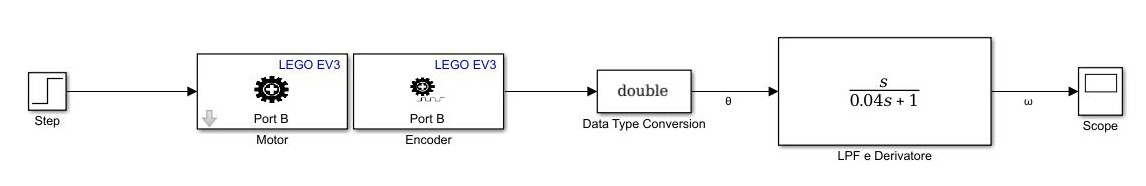
\includegraphics[width=\textwidth]{motoreSimulink.jpg}
	\caption{Schema a blocchi Motore}
	\label{motoreSimulink}
\end{figure}
\noindent Il LEGO MINDSTORMS EV3 è dotato di un motore, l'EV3 Large Servo Motor, la cui velocità angolare, misurata in $deg/s$, è stata assunta come uscita del sistema.\\
I valori di ingresso accettabili sono compresi tra -100 e +100, dove $\pm$100 corrispondono alla massima potenza erogabile in entrambi i versi di rotazione.

Al fine di riuscire a modellarlo, abbiamo applicato al motore un albero dotato di pesi posti a una certa distanza dallo stesso in modo tale da incrementarne il momento d'inerzia $I$. Questo poiché in assenza di un carico significativo la dinamica del motore risulta  troppo veloce per  essere identificata con gli strumenti a nostra disposizione. In particolare l'insufficiente precisione e la limitata frequenza massima di campionamento dell'encoder non permettono una corretta analisi del transitorio del motore. Al fine di ridurre il più possibile l'errore è stato scelto come tempo di campionamento dell'encoder il valore minimo supportato: 0.001$s$.\\
Come conseguenza all'aggiunta del carico, si ha una diminuzione dell'accelerazione angolare massima $\alpha$ in accordo con la seconda legge di Newton (in forma angolare) $\tau = I\alpha$, dove $\tau$ è il momento della forza o, più semplicemente, la coppia massima erogata, valore caratteristico del motore.
\begin{figure}[ht]
	\centering
	\includegraphics[width=\textwidth]{megainerzia.png}
	\caption{Carico per aumentare Inerzia del motore}
	\label{megainerzia}
\end{figure}
\\In questo modo il tempo di assestamento $t_a$ del sistema è sensibilmente più lungo ed è dunque possibile trovare una funzione di trasferimento assimilabile a quella dell'EV3 Large Servo Motor.

All'interno del motore, come già accennato, è presente un encoder che permette di misurare, in gradi, la posizione angolare $\theta$ dello stesso.
Perciò, al fine di ottenere la velocità angolare $\omega$, è stato applicato in cascata un derivatore, e per introdurre il polo necessario alla realizzabilità del blocco, un filtro passa basso con frequenza di taglio $\omega_c=25rad/s$. \\Quest'ultimo è indispensabile per attenuare le alte frequenze della risposta del sistema, dovute alla derivazione del segnale campionato, affinché la funzione in uscita sia meno spezzata possibile e, di conseguenza, più facilmente identificabile.\\
In prima analisi si è scelto un filtro con un $\omega_c$ più elevata, ovvero $100rad/s$, in modo che la costante di tempo non influenzasse la dinamica del motore stesso.
Il risultato che si ottiene sotto tali condizioni, utilizzando come ingresso una funzione gradino con valore finale pari a 50, è mostrato nella figura \ref{motore50StepCamp1000Polo100}.
\begin{figure}[ht]
	\centering
	\includegraphics[width=\textwidth]{motore50StepCamp1000Polo100.png}
	\caption{Risposta al gradino con $\omega_c=100rad/s$ }
	\label{motore50StepCamp1000Polo100}
\end{figure}
\\E' evidente come la frequenza di taglio scelta per il filtro non sia sufficiente ad eliminare le alte frequenze dell'uscita per cui, procedendo gradualmente siamo giunti a  scegliere una frequenza $\omega_c = 25rad/s$ con la quale l'uscita del sistema diventa accettabile (figura \ref{motore50StepCamp1000}).
\begin{figure}[ht]
\centering
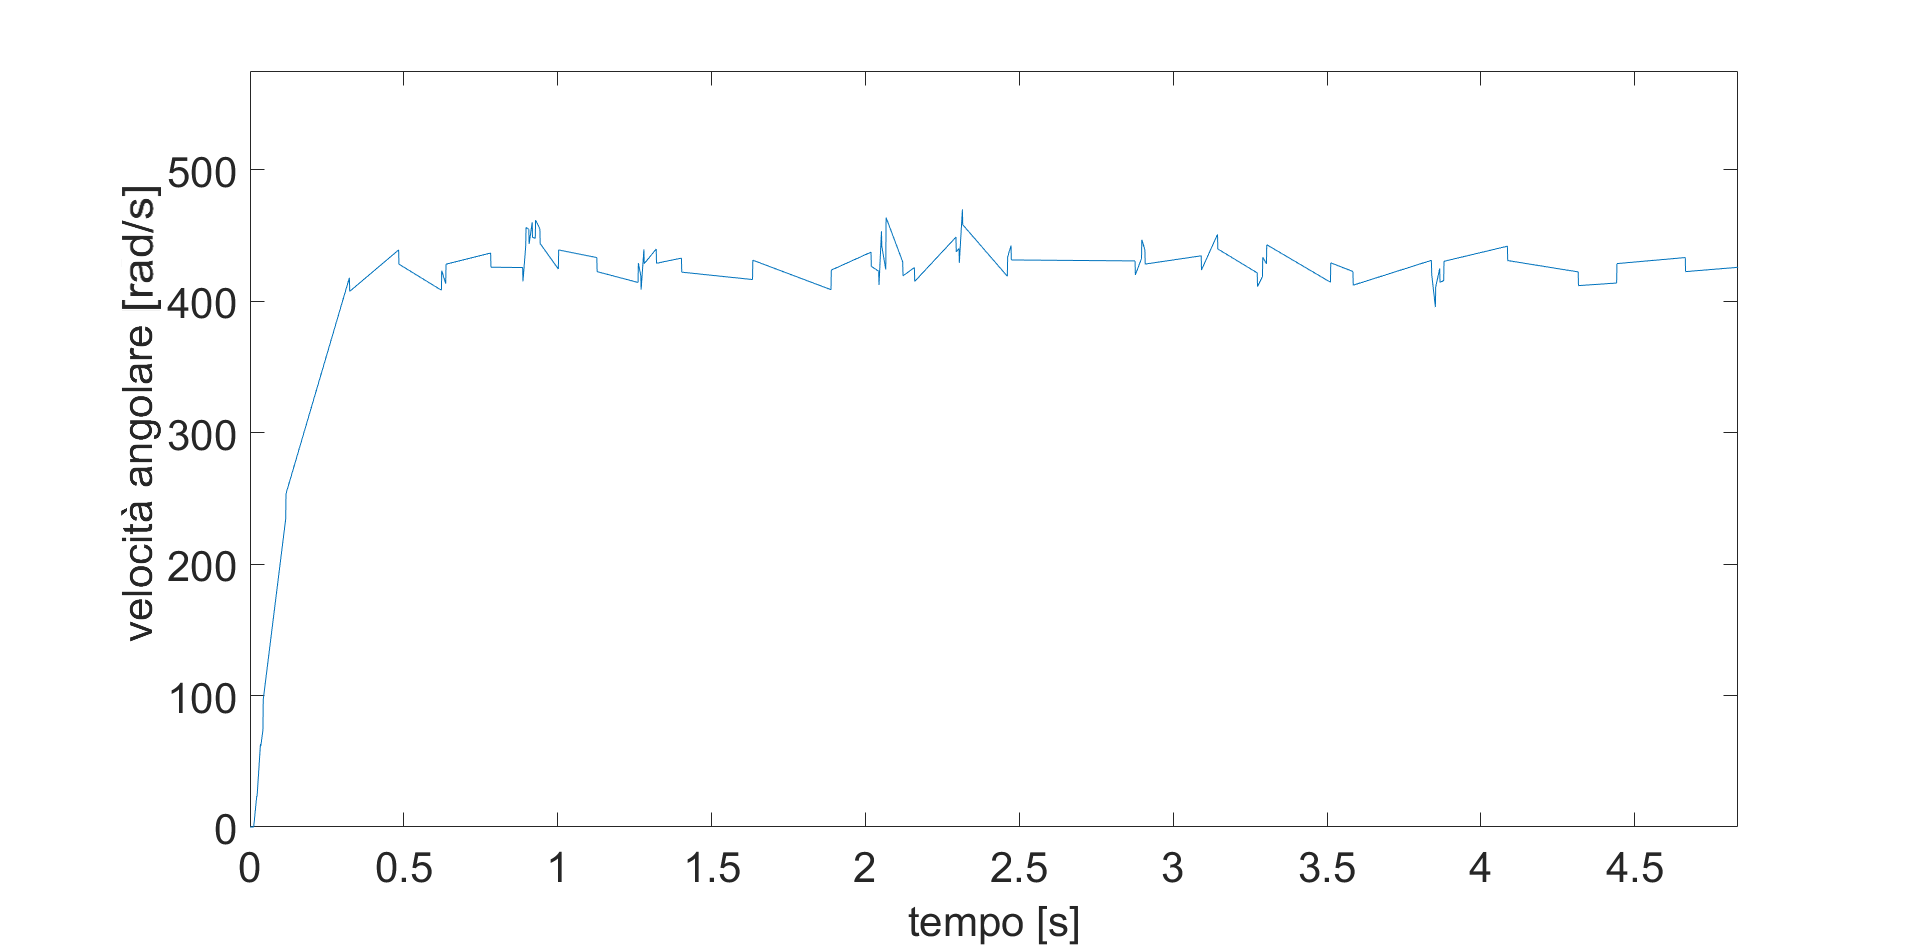
\includegraphics[width=\textwidth]{motore50StepCamp1000.png}
\caption{Risposta al gradino con $\omega_c=25rad/s$}
\label{motore50StepCamp1000}
\end{figure}
Prendendo quindi in esame quest'ultimo grafico è evidente che sia possibile approssimare la funzione di trasferimento del motore come una funzione del $\ang{1}$ ordine la cui `forma campione' è data dalla formula $$T(s)=\displaystyle\frac{k}{1+s\tau}$$ \\
Abbiamo quindi stimato una costante di tempo $\tau$ (tempo che impiega la funzione a raggiungere il 63.2\% del valore di regime) del sistema pari a circa 0.15$s$ e guadagno statico $k$ di 10.4.\\
La funzione di trasferimento che ne consegue è dunque:
\\
$$
T_{motore}(s)=\displaystyle\frac{10.4}{0.15s+1}
$$
\\
In figura \ref{modMotorvsReale} un confronto tra $T_{motore}(s)$ e la funzione di trasferimento reale del motore.
\begin{figure}[ht]
	\centering
	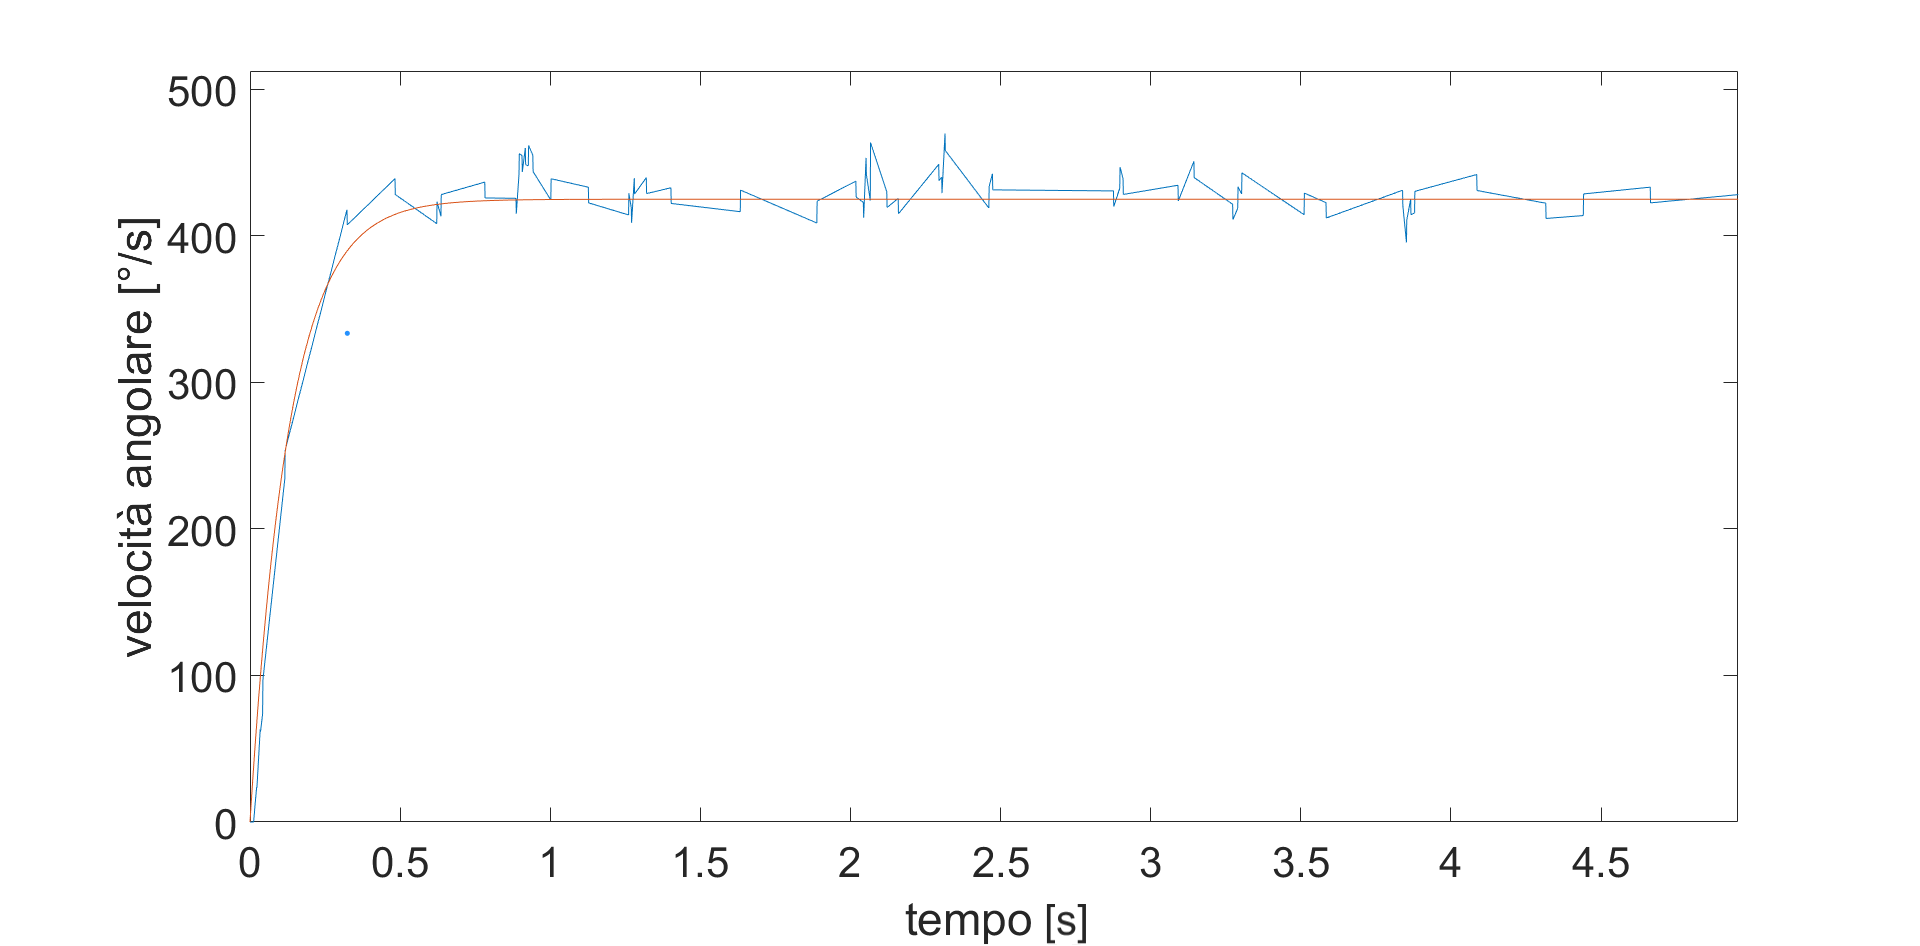
\includegraphics[width=\textwidth]{modMotorvsReale.png}
	\caption{Risposta al gradino del Motore reale e del suo modello}
	\label{modMotorvsReale}
\end{figure}

\section{Dalla velocità angolare alla coppia}
È necessario ora ottenere la coppia generata dal motore in funzione del tempo al fine di utilizzarla come ingresso per la funzione di trasferimento del pendolo la quale sarà trattata in modo approfondito nel capitolo \ref{PendCarrello}.\\
L'equazione fisica utilizzata per calcolare tale coppia è la seguente:
$$
\tau=K\omega+I\alpha
$$
dove il primo termine indica appunto la coppia, mentre i restanti due sono rispettivamente l'attrito interno al motore e il momento torcente.
Più nello specifico $K$ rappresenta il coefficiente di smorzamento viscoso misurato in $N\cdot m\cdot s/deg$, $\omega$ la velocità angolare, $I$ il momento d'inerzia$^{[1]}$ del sistema e $\alpha$ l'accelerazione angolare.

Calcoliamo innanzi tutto 
$$
I=3M_Rd_R^2+3M_rd_r^2+3I_a+3I_A+\displaystyle\frac{m_ar^2}{2}
$$
nella quale i primi due termini indicano i momenti d'inerzia delle sei ruote, il terzo e il quarto quelli delle sei aste che collegano le ruote all'albero, mentre l'ultimo termine rappresenta il momento d'inerzia dell'albero (asta centrale). Nel calcolo dell'inerzia di ogni componente si sono ovviamente fatte le approssimazioni del caso: le aste sono state considerate omogenee e di sezione circolare, le ruote, masse puntiformi concentrate nel loro centro di massa.\\
Per calcolare l'inerzia delle sei aste utilizziamo il teorema di Huygens-Steiner$^{[1]}$, o degli assi paralleli:
$$
I=I_{cdm}+m_{asta}d^2
$$
Dove $d$ è la distanza tra l'asse passante per il centro di massa e quello parallelo di rotazione (rispetto al quale calcoliamo il momento).\\
$$
I_{asta}=\displaystyle\frac{1}{12}m_{asta}l^2+m_{asta}(\displaystyle\frac{l}{2})^2=\displaystyle\frac{1}{3}m_{asta}l^2
$$
Inserendo ora i parametri misurati  e riportati nella tabella \ref{Inerzia}, si ricava un momento d'inerzia $I$ pari a 0.001364 $Kg\cdot m^2$.
\begin{table}[ht]
	\begin{tabular}{|l|l|l|l|}
		\hline
		\textbf{Sigla} & \textbf{Valore} & \textbf{U.d.m.} & \textbf{Parametro}\\
		\hline
		$M_R$ & 0.0395 & $kg$ & massa ruota grande\\
		\hline
		$M_r$ & 0.023 & $kg$ & massa ruota piccola\\
		\hline
		$m_a$ & 0.0015 & $kg$ & massa asta corta\\	
		\hline
		$m_A$ & 0.002 & $kg$ & massa asta lunga\\	
		\hline
		$l_a$ & 0.068 & $m$ & lunghezza asta corta\\
		\hline
		$r$ & 0.002 & $m$ & raggio asta\\
		\hline
		$l_A$ & 0.091 & $m$ & lunghezza asta lunga\\
		\hline
		$d_r$ & 0.061 & $m$ & distanza ruota piccola - asse di rotazione\\
		\hline
		$d_R$ & 0.085 & $m$  & distanza ruota grande - asse di rotazione\\
		\hline
	\end{tabular}
\caption{Parametri del carico dell'albero motore}
\label{Inerzia}
\end{table}

Essendo $\tau=K\omega+I\alpha$ possiamo disegnare tramite Simulink il diagramma a blocchi rappresentato in figura \ref{modMotoreTorque}:
\begin{figure}[ht]
	\centering
	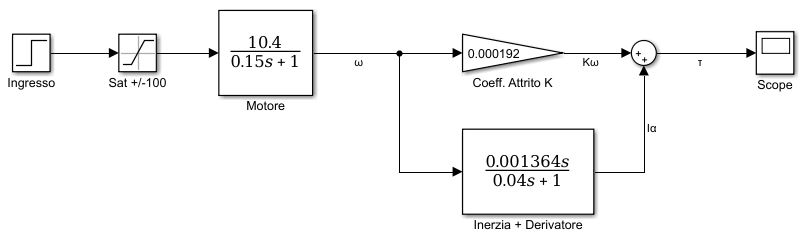
\includegraphics[width=\textwidth]{modMotoreTorque.jpg}
	\caption{Modello completo del Motore$^{[6]}$}
	\label{modMotoreTorque}
\end{figure}
\\L'uscita del sistema è proprio la coppia $\tau$ desiderata.\\
Si può notare come nel blocco inferiore siano stati aggiunti il derivatore e il filtro passa-basso già utilizzati in precedenza per ricavare la velocità dalla posizione. Il primo è necessario dal momento che l'accelerazione angolare $\alpha$ è proprio la derivata della velocità angolare $\omega$. Per quanto riguarda il filtro, invece,
il discorso è analogo a quello trattato in precedenza:
è stato aggiunto (scegliendo appositamente una frequenza di taglio abbastanza alta da non alterare la dinamica del sistema) siccome un derivatore puro sarebbe stato fisicamente irrealizzabile (funzione impropria).\\
Inoltre si è resa necessaria anche l'aggiunta di un blocco di saturazione dell'ingresso dal momento che, come già reso noto in precedenza, l'EV3 Large Servo Motor accetta valori compresi tra -100 e +100 considerando quelli esterni a tale intervallo coincidenti con gli estremi.\\
In ultimo il valore di $K$, unico parametro incognito rimasto, è stato invece ricavato sperimentalmente avendo nota dalle specifiche LEGO$^{[5]}$ la coppia massima a regime dell'EV3 Large Servo Motor $\tau_{reg}=0.2N\cdot m$.\\
Come mostrato in figura \ref{torque02} un valore di K pari a 0.000192 $Nm\cdot s/deg$ per un ingresso a gradino con valore finale 100 consente di rispettare appieno tale specifica.
\begin{figure}[ht]
	\centering
	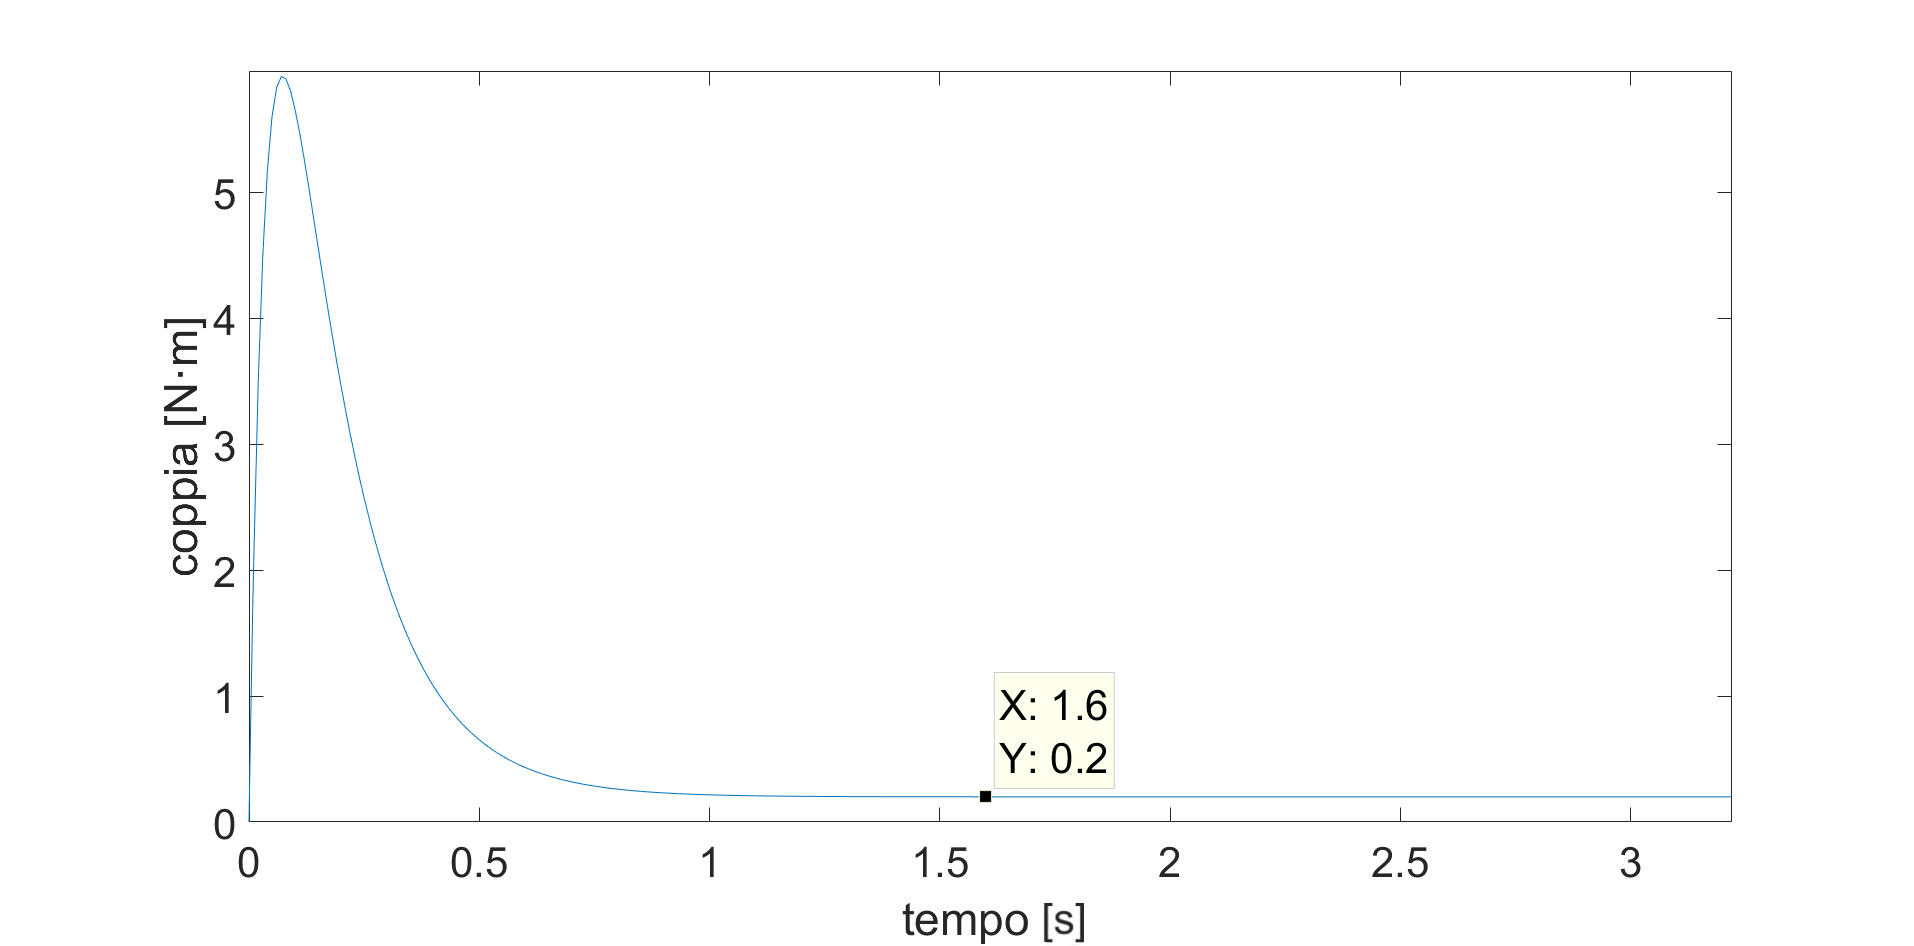
\includegraphics[width=\textwidth]{torque192.png}
	\caption{Risposta al gradino del modello completo}
	\label{torque02}
\end{figure}